\subsection{Current from stimulus}

This section describes the process of converting a luminance stimulus into current. The process begins by converting the luminance to local contrast. This local contrast is then converted to a frequency in the gamma band. Finally, the relationship between the frequency and the current is determined and used to convert the frequency into current.

\subsubsection{From luminance to contrast}

To transform the stimulus patch $\patchmatrix$ to the patch of PING networks in V1, we apply the lattice of size $n \times n$, such that each oscillatory network contains a field of $m \times m$ pixels. An example of the resulting lattice is displayed in Figure \ref{fig:llc-lattice-example}.


\begin{figure}[!htp]
    \centering
    \begin{subfigure}[t]{0.4\textwidth}
        \centering
        \newcommand{\splw}{\textwidth}
\newcommand{\splh}{\splw}

\newcommand{\splnrverticallines}{11}
\newcommand{\splverticalinterval}{0.08333} % 1 / (splnrverticallines + 1)

\newcommand{\splnrhorizontallines}{11}
\newcommand{\splhorizontalinterval}{0.08333}

\begin{tikzpicture}[
    cline/.style = {very thick, color-one},
]
    \begin{scope}
        \node[anchor=south west,inner sep=0] at (0,0) {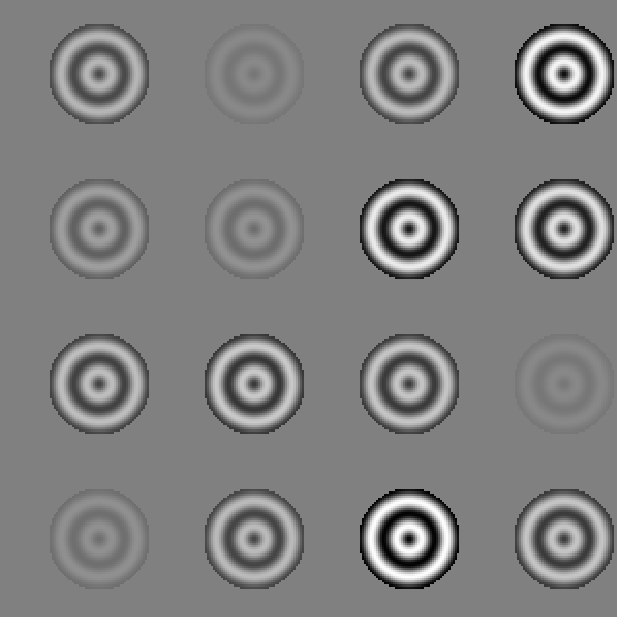
\includegraphics[width=\splw]{src/assets/images/stimulus-patch-lattice.png}};
        
        % vertical
        \foreach \i in {1, 2, ..., \splnrverticallines}{
            \draw[cline] (\i * \splverticalinterval * \splw, 0) -- (\i * \splverticalinterval * \splw, \splh) {};
        }
        
        % horizontal
        \foreach \i in {1, 2, ..., \splnrverticallines}{
            \draw[cline] (0, \i * \splhorizontalinterval * \splh) -- (\splw, \i * \splhorizontalinterval * \splh) {};
        }

    \end{scope}
\end{tikzpicture}
        \caption{A 20 $\times$ 20 lattice applied to a patch.}
        \label{fig:llc-lattice-example}
    \end{subfigure}
    \hspace{0.06\textwidth}
    \begin{subfigure}[t]{0.4\textwidth}
        \centering
        
\includegraphics[width=\textwidth]{src/assets/images/local-contrast.png}
        \caption{Local contrasts of the patch in Figure \ref{fig:llc-lattice-example}: $0$ (black) $\to$ $1$ (white).}
        \label{fig:llc-local-contrast-example}
    \end{subfigure}
    \caption[Patch lattice and local contrast]{The lattice of a patch and its vertices' local contrasts. 
    The patch was generated with the parameters $\anndistscale = 1.5$, $\contrange = 1$.}
    \label{fig:lattice-local-contrast-example}
\end{figure}


Let $\pingnets$ be the set containing the PING networks. Let $\pix: \pingnets \to (\mathbb{Z}_+)^{2 \times m^2}$ be a function mapping a network to the set of all $m^2$ pixel coordinates it contains.
For each network $\pingnet \in \pingnets$, a local contrast $\LC: V \to \mathbb{R}$ is the weighted root-mean-squared (RMS) contrast defined as follows \cite{Frazor2006}:
\begin{equation}
    \LC_\pingnet = \sqrt{
        \frac{
            \sum_{(i, j) \in \patchmatrix} \weight_{\pingnet, (i, j)} \frac{(\patchmatrix_{i, j} - \overline{\fullmatrix})^2}{\overline{\fullmatrix}^2}
        }{
            \sum_{(i, j) \in \patchmatrix} \weight_{\pingnet, (i, j)}
        }
    },
\end{equation}
\begin{comment}
\begin{equation}
    \LC_\pingnet = \sqrt{
        \frac{
            \sum_{(i, j) \in \pix(\pingnet)} \weight_{\pingnet, (i, j)} \frac{(\patchmatrix_{i, j} - \overline{\fullmatrix})^2}{\overline{\fullmatrix}^2}
        }{
            \sum_{(i, j) \in \pix(\pingnet)} \weight_{\pingnet, (i, j)}
        }
    },
\end{equation}
\end{comment}
where $\overline{\fullmatrix}$ is the mean over all luminance values in $\fullmatrix$, and $\weight: \pingnets, \mathbb{N}^2 \to \mathbb{R}$ is the weight of a pixel with respect to a network, as shown in Equation (\ref{eq:weight-pixel-network}). An example of a local contrast matrix can be seen in Figure \ref{fig:llc-local-contrast-example}.

To define that weight, one first needs to complete a number of steps.
Let $\centr : \pingnets \to \mathbb{R}_+^2$ be the function mapping a particular PING network in the patch to the location of its center. As the center of the gaze (fovea) coincides with the center of the stimulus, the eccentricity $\ecc: \pingnets \to \mathbb{R}_+$ in degrees for a network $v \in \pingnets$ is
\begin{equation}
\begin{gathered}
    \ecc_{\pingnet} = \frac{1}{\atopix} \cdot \left\| \stimcenter, \ \patchstart + \centr(\pingnet) \right\|, \\
    \stimcenter = \left( \frac{\fullwidth}{2}, \frac{\fullheight}{2}   \right).
\end{gathered}
\end{equation}

Let $\slopeRF \in \mathbb{R}$ be the slope, the ratio of receptive field diameter to eccentricity, and $\interceptRF \in \mathbb{R}$ - the intercept \cite{Freeman2011, MaryamPLACEHOLDER}.
Let $\diamRF_{\min} \in \mathbb{R}_+$ be smallest allowed diameter of the receptive field.
Then, the diameter of the receptive field $\diamRF \in \mathbb{R}$ of $\pingnet$ is 
\begin{equation}
    \diamRF_\pingnet = \max{( \slopeRF \cdot \ecc_\pingnet + \interceptRF, \ \diamRF_{\min} )}.
\end{equation}

Let $\stdrf: \pingnets \to \mathbb{R}$ be the standard deviation of the receptive field diameter of a Gaussian beam \cite{MaryamPLACEHOLDER}. It can be obtained by utilizing the full width at half maximum $\fwhm: \pingnets \to \mathbb{R}$ in the following way:
\begin{equation}
    \begin{cases}
        \fwhm_\pingnet = \sqrt{\frac{\ln(2)}{2}} \cdot \diamRF_\pingnet \\
        \fwhm_\pingnet = 2 \sqrt{2 \ln(2)} \cdot \stdrf_\pingnet
    \end{cases}
    \Rightarrow 
    \stdrf_\pingnet = \frac{1}{4} \diamRF_\pingnet.
\end{equation}

Having derived the standard deviation, the weight of the pixel $i, j \in \{ 0, 1, \cdots, \patchsize - 1 \}$ with respect to a PING network $\pingnet$ can be defined at last. This value is specific to each network as it reflects its unique receptive field modeled with an isotropic 2D Gaussian function \cite{MaryamPLACEHOLDER}:
\begin{equation}
    \weight_{\pingnet, (i, j)} = \exp \left(
        -\frac{\left( \frac{1}{\atopix} \cdot \| (i, j), \ \centr(\pingnet) \|\right)^2}{ 2 \stdrf_\pingnet^2 }
    \right).
    \label{eq:weight-pixel-network}
\end{equation}
\subsubsection{From contrast to frequency}

Now, the oscillation frequency $f$ of the PING network $\pingnet$ can be obtained through the local contrast:
\begin{equation}
    f_\pingnet = 25 + 0.25 \cdot \LC_\pingnet.
\end{equation}
These relations reflect the typical gamma frequency of a neural network in V1.
\subsubsection{From frequency to current}

This section describes a method for determining the relationship between gamma frequencies and input currents. It involves simulating the network using the Izhikevich model with different currents and constructing a time-frequency representation (TFR) of the resulting spike trains using the Morlet wavelet transform. The dominant frequency of gamma oscillations in the signal can be determined from the TFR. The dominant frequency for each simulation is then plotted against the corresponding input current to find the relationship between current and frequency.

\paragraph{Simulating with different currents}

To collect the required data for a given input current, we simulate the Izhikevich model with the previously introduced parameters (see Section \ref{sec:grid-network}). Instead of the current input from an external stimulus, $I_\stim$ in Equation (\ref{eq:current-components}), current $I_\inpt$ is used:
\begin{equation}
    I_{\inpt, v} = \begin{cases}
        \meancurrent_\ex & \text{ if } \type(v) = \ex \\
        \meancurrent_\inh & \text{ if } \type(v) = \inh
    \end{cases}.
\end{equation}
The input current to inhibitory neurons $\meancurrent_\inh$ is fixed for all simulations at $4.0$, while the input to excitatory neurons $\meancurrent_\ex$ is modulated per simulation. The 26 simulations are performed for the values $\meancurrent_\ex = \{ 0, 2, 4, \cdots, 50 \}$.

Equation (\ref{eq:Izhikevich-model-p30}) allows for the detection of spikes and, thus, the construction of spike trains, i.e., the sequence of neuronal firing times. For a neuron $v \in V$, the spike train $\spiketrain \in \{0, 1\}^{|\timesteps|}$ can be defined as follows:
\begin{equation}
    \spiketrain_v = 
    \left( 
        \timespiked_{v, \timesteps_i}
    \right)_{\timesteps_i \in \timesteps},
\end{equation}
where the function $s: \{V, \timesteps\} \to \{0, 1\}$ returns $1$ if neuron spikes at a particular time, and otherwise returns $0$:
\begin{equation}
    \timespiked_{v, \timesteps_i} = \begin{cases}
        1 &\text{ if } p_v(\timesteps_i) \geq p_\peak
        , \\
        0 &\text{ otherwise}.
    \end{cases}
\end{equation}

As mentioned in Section \ref{sec:grid-ping}, the simulation time has been chosen to be $1000$ ms.
For the purposes regarding the Fast Fourier Transform (FFT) algorithm, as discussed in the next paragraph, let $\offset \in \mathbb{N}$ be equal to $296$.

Let $\tfrsimulations$ be a set of the 26 simulations, each associated with a particular value of $\meancurrent_\ex$. Let $\tfrsimulation \in \tfrsimulations$ be one of these simulations. A time-dependent signal $\spikesignal \in \{0, 1\} ^ {|V| \ \times \ (|\timesteps| - \offset)}$ is created by discarding the first $\offset$ time steps from each neuron's spike train obtained during the simulation $\tfrsimulation$.


\paragraph{Finding dominant frequencies from TFR}

This thesis is concerned with gamma oscillations ($25 - 80$ Hz). Let $\gammafreq \in \mathbb{N}^{55}$ be a sequence of integer frequencies in the gamma range:
\begin{equation}
    \gammafreq = \left<
    25, 26, \cdots, 80
    \right>.
\end{equation}
For a signal with a given input current, the corresponding frequency that said signal triggers is the most prominent within the gamma band. To analyze the frequency behavior of a signal, one needs to construct its time-frequency representation (TFR). 
The TFR encodes the energy of the signal as a function of time and frequency and is used to determine the dominant frequency of gamma oscillations in the signal.
To compute the TFR using the Morlet wavelet transform, the steps outlined below are to be performed.

\begin{enumerate}
    \item The time axis for the Morlet wavelet $\morlettime \in [-1, 1]^{2001}$ is defined as a sequence of values spaced $0.001$ seconds apart, from -1 to 1:
    \begin{equation}
        \morlettime = \left<
        -1, -0.999, \cdots, 1
        \right>.
    \end{equation}

    \item The discrete Fourier transform (DFT) of the spike train signal $\ft\spikesignal_\tfrsimulation \in \mathbb{C}^{\nconv}$ is computed using the Fast Fourier Transform (FFT) algorithm. The length of the signal is increased by zero-padding to $\nconv \in \mathbb{N}$:
    \begin{equation}
        \nconv \leftarrow \nconv_\tfrsimulation = |\spikesignal_\tfrsimulation| + |\morlettime| - 1.
    \end{equation}
    Computing $\nconv$ in such a way ensures that the resulting length is a power of two and, therefore, is suitable for use in the FFT.
    In the present case, $\nconv = 2704 = 52^2$ due to the value of $\offset$ defined earlier.
    The values of $\nconv$ do not need to be computed for each simulation as $|\spikesignal_\tfrsimulation|$ does not change.

    \item The edge indices later used to remove the zero-padding $\halfwave \in \mathbb{N}^2$ are computed:
    \begin{equation}
        \halfwave
        = 
        (\halfwave_\substart, \halfwave_\subend) 
        =
        \left(
            \floor{
                \frac{
                    |\morlettime| - 1         
                }{2}
            },
            |\nconv| - \floor{
                \frac{
                    |\morlettime| - 1         
                }{2}
            }
        \right).
    \end{equation}

    \item For each gamma frequency $\onegammafreq \in \gammafreq$, a Morlet wavelet $\morlet \in \mathbb{C}^{|\morlettime|}$ is constructed as a complex sinusoid modulated by a Gaussian window. The width $\gausswidth \in \mathbb{R}$ of the Gaussian can be adjusted to change the shape of the wavelet. The wavelet is thus defined as follows:
    \begin{equation}
        \morlet_{\onegammafreq, j} = 
        \underbrace{
            \exp \left(
            \complexi \cdot 2 \pi \cdot \onegammafreq \cdot \morlettime_j
            \right)
        }_{\text{complex sinusoid}}
        \cdot
        \underbrace{
            \exp \left(
                - \frac{
                    \morlettime_j^2
                }{
                    2 \cdot \gausswidth^2
                }
            \right),
        }_{\text{Gaussian window}}
    \end{equation}
    where $\complexi$ is the imaginary unit (boldface for readability and to distinguish from the index $i$).
    
    \item The normalized DFT of each Morlet wavelet $\overline{\ft\morlet}_{\onegammafreq} \in \mathbb{C}^{\nconv}$ is computed:
    \begin{equation}
        \overline{\ft\morlet}_{\onegammafreq} = 
        \frac{
            {\ft}{\morlet_{\onegammafreq}}
        }{
            \max \left(
                {\ft}{\morlet_{\onegammafreq}}
            \right)
        }.
    \end{equation}

    \item For each simulation, the DFT of each Morlet wavelet is multiplied element-wise by the DFT of the spike train signal ($\ft{\morlet_{\onegammafreq}}$ multiplied by $\ft\spikesignal_\tfrsimulation$). This produces a new frequency-domain representation of the signal that encodes its frequency content at each point in time.

    \item The product of the DFTs is inverse-transformed back into the time domain using the Inverse Fast Fourier Transform (IFFT) algorithm. Let the result be $\tmp \in \mathbb{C}^\nconv$.
    
    \item The resulting time-domain signal is trimmed to remove the parts that were added by zero-padding with $\halfwave$ and is used to construct the TFR of the signal. Then the TFR $\left( \tfr \in \mathbb{C}^{ |\gammafreq| \ \times \ |\spikesignal_\tfrsimulation|} \right)$ for the simulation $\tfrsimulation$ is
    \begin{equation}
        \tfr_{\tfrsimulation, \onegammafreq} 
        = 
        \left< 
            \tmp_{\tfrsimulation, \onegammafreq, \halfwave_i} 
            \ \mid \ 
            \halfwave_\substart \leq \halfwave_i < \halfwave_\subend
        \right>.
    \end{equation}
    
    \item The TFR is analyzed to establish the dominant frequency of gamma oscillations in the signal. In particular, the signal's most prominent frequency $\domgammafreq \in \gammafreq$ is determined by computing the mean of the TFR magnitudes (absolute values) along the frequency dimension and finding the frequency at which the resulting number is the largest:
    \begin{equation}
    \begin{gathered}
        \domgammafreq_\tfrsimulation = \arg \max_\onegammafreq \left(
            \meanabsval\_\tfr_{\tfrsimulation}
        \right),
        \\
        \meanabsval\_\tfr_{\tfrsimulation, \onegammafreq} = 
        \frac{
            \sum_{i=0}^{|\spikesignal_\tfrsimulation| - 1} 
            |\tfr_{\tfrsimulation, \onegammafreq, i}|
        }{
           |\spikesignal_\tfrsimulation|
        }.
    \end{gathered}
    \end{equation}
\end{enumerate}


\paragraph{Discovering frequency-current relationship}

For each current input strength to excitatory neurons, the most prominent frequency is now known. Thus, the relationship can be analyzed and extrapolated. By plotting frequencies against currents, it can be observed that they follow a linear relationship (see Figure ???). Thus, the Theil–Sen estimator can fit a predictive model for the observed data. This regression method has been chosen as it is robust against outliers and does not require the assumption of normally distributed errors. 

\begin{figure}[!htp]
    \centering
    % ----- INPUT
\newcommand{\fcimagew}{0.45\textwidth}
\newcommand{\fcimageh}{\fcimagew}

% to shift for ticks
\newcommand{\fcshiftx}{1.3em}
\newcommand{\fcshifty}{1em}

% to shift to the middle from kinda the middle
\newcommand{\fcmidshiftx}{0.5em}
\newcommand{\fcmidshifty}{0.4em}

%
\newcommand{\fchormid}{0.5 * \fcimagew}
\newcommand{\fcvermid}{0.5 * \fcimageh}



\begin{tikzpicture}[
        arr/.style = { -{Stealth[ ]} },
        bluearrow/.style = {arr, draw=third-color, fill=third-color, thick},
        blackarrow/.style = {arr, ultra thick},
    ]
    
    \begin{scope}

        \node[
            shift={(\fcmidshiftx, -\fcshifty)}
        ] at (\fchormid, 0) {{ \small Current}};
        
        \node[
            shift={(-\fcshiftx, \fcmidshifty)},
            rotate=90
        ] at (0, \fcvermid) {{\small Frequency}};

        
        % \node[shift={(\apwest, \apshifth)}, anchor=west] at (0, \appeakh) {peak};
        
    \end{scope}
    
    \begin{scope}
        \node[anchor=south west,inner sep=0] at (0,0) {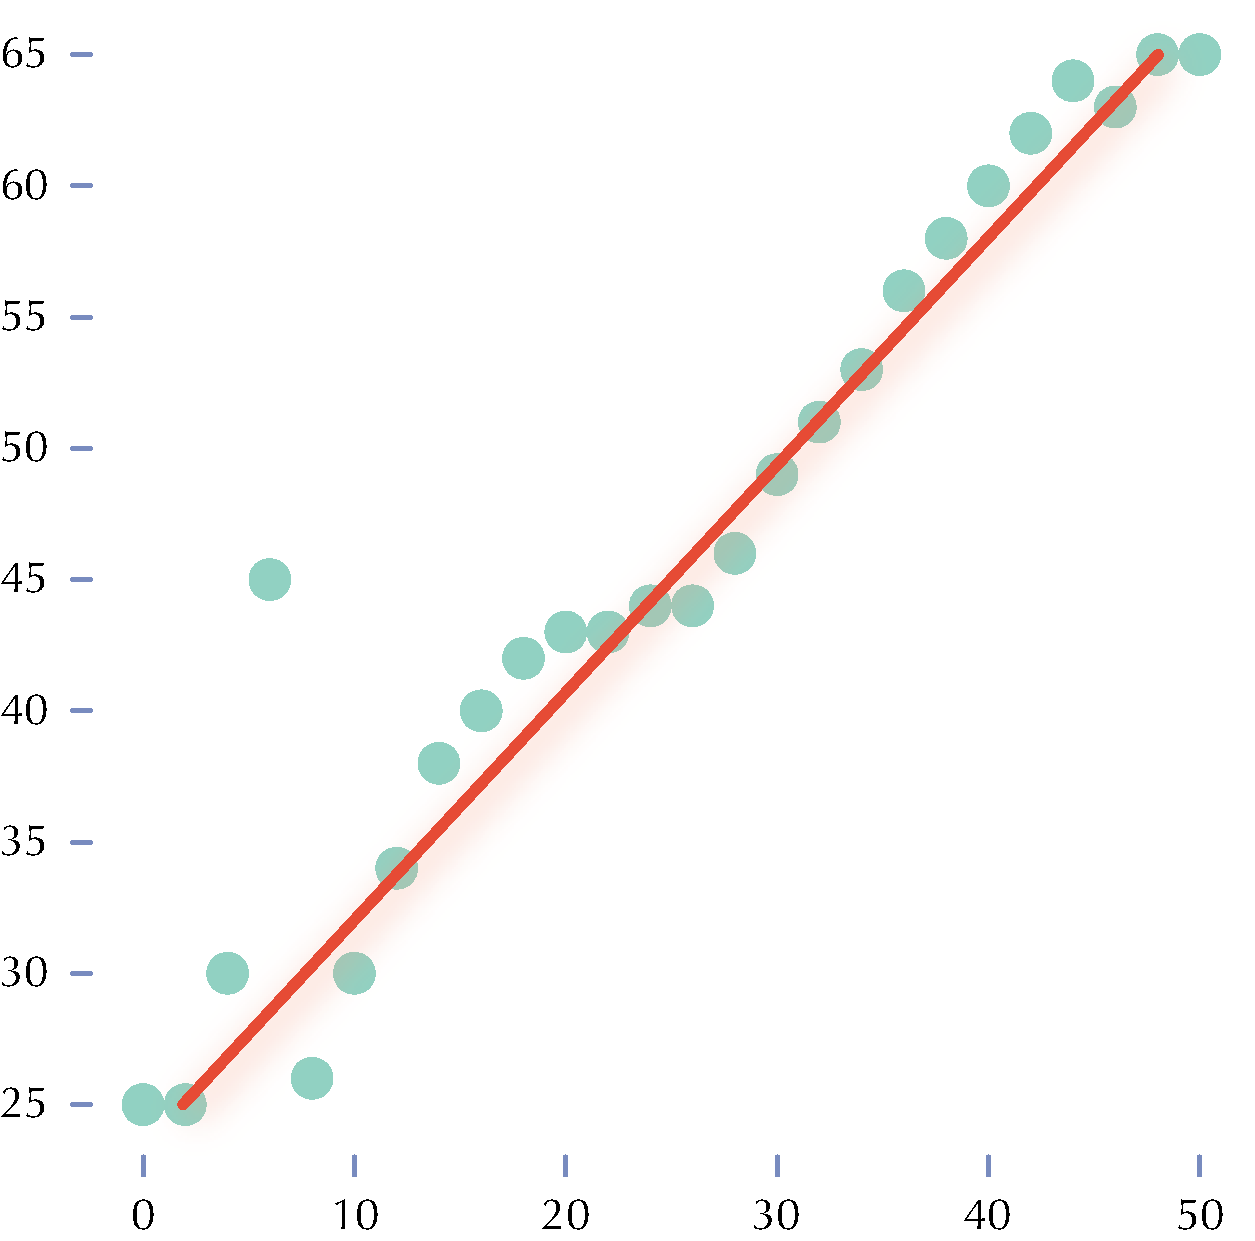
\includegraphics[width=\fcimagew]{src/assets/images/f-c-relationship.pdf}};
    \end{scope}
        
\end{tikzpicture}
    \caption{Caption}
    \label{fig:my_label}
\end{figure}

The Theil–Sen estimator defines the slope of the fitted line $\fcslope \in \mathbb{R}$ as the median of all possible slopes between pairs of points from the frequency-current graph:
\begin{equation}
    \fcslope = \median_{
        \tfrsimulation_i, \tfrsimulation_j \in \tfrsimulations \times \tfrsimulations
    } \left( 
        \frac{
            \domgammafreq_{\tfrsimulation_i} - \domgammafreq_{\tfrsimulation_j}
        }{
            I_{\ex, \tfrsimulation_i} - I_{\ex, \tfrsimulation_j}
        } 
    \right)
\end{equation}
To compute the intercept $\fcintercept \in \mathbb{R}$, the estimator uses the average values along the axes and the previously computed slope:
\begin{equation}
    \fcintercept = 
    \frac{1}{|\tfrsimulations|}
    \sum_{\tfrsimulation \in \tfrsimulations}
    \domgammafreq_\tfrsimulation
    -
    \frac{\fcslope}{|\tfrsimulations|}
    \sum_{\tfrsimulation \in \tfrsimulations}
    I_{\ex, \tfrsimulation}
\end{equation}

Knowing the slope of the linear relationship between the frequency and current, the current from external stimulus to the excitatory neurons in a PING network $\pingnet$ can be defined as follows:
\begin{equation}
    I_{\stim, \pingnet} = \fcslope \cdot f_\pingnet + \fcintercept.
\end{equation}
The derived values for $\fcslope$ and $\fcintercept$ are shown in Table ???.

\todo{include table ??? and figure ???}